\appendix
\section{Приложения}

\begin{frame}
\frametitle{Технологический стек}
\begin{itemize}
    \item Операционная система \textit{Ubuntu 20.04 LTS}
    \item Язык программирования \textit{Python 3.8.12}
    \item База данных \textit{PostgreSQL 12} с расширением \textit{PostGIS 3.1}
    \item Веб-сервер \textit{nginx}
    \item Автоматическое развертывание \textit{Gitlab-CI}
    \item Контейнеризация \textit{Docker} и \textit{docker-compose}
    \item Документация \textit{OpenAPI} и \textit{LaTex}
    \item Система сборки логов \textit{ELK}
    \item Протоколы взаимодействия \textit{REST API over HTTP}
    \item Формат данных \textit{JSON}
\end{itemize}
\end{frame}

\begin{frame}
\frametitle{Диаграмма развёртывания}
\begin{figure}
    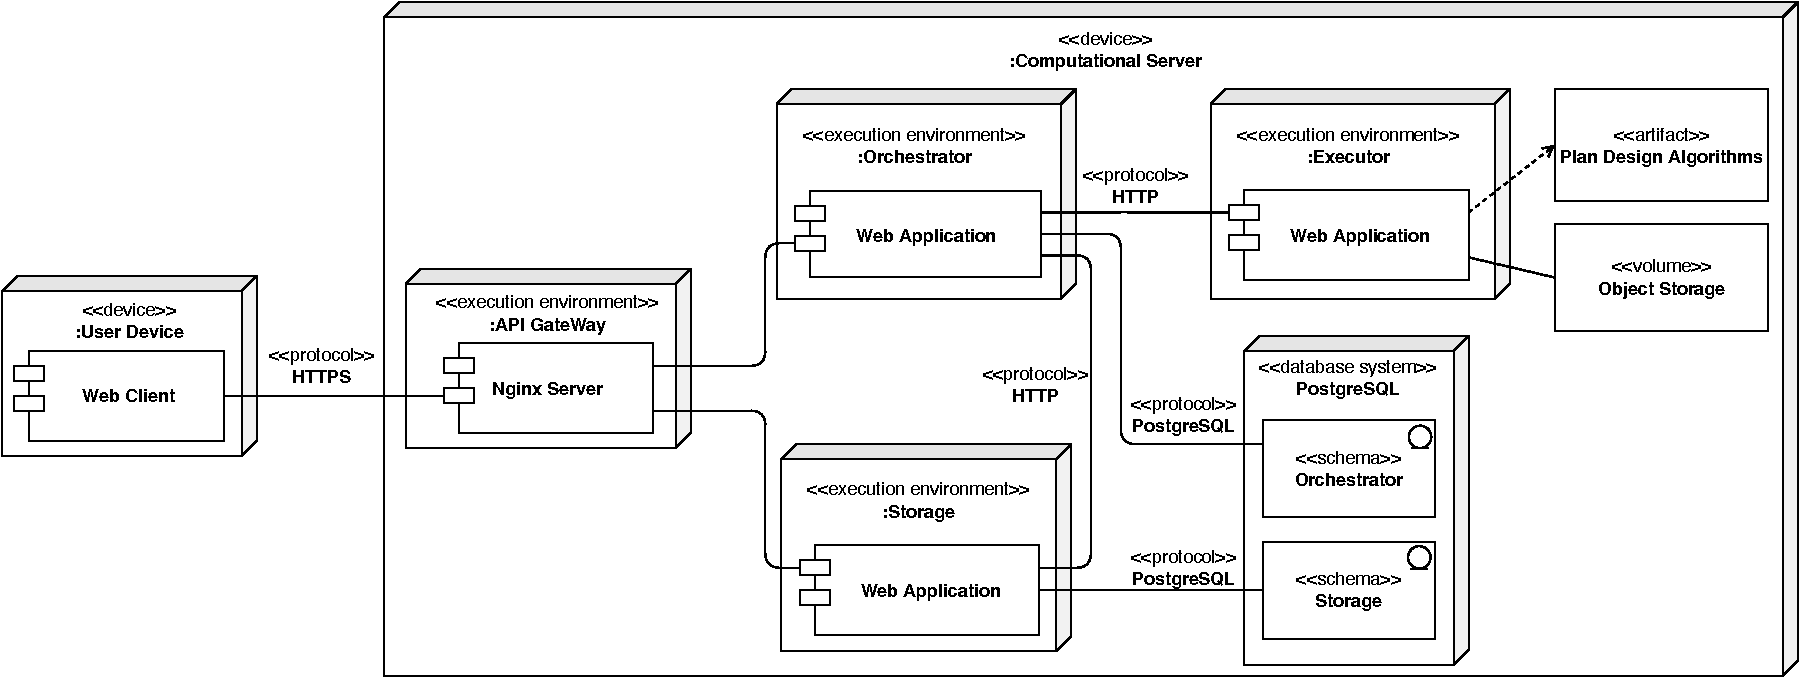
\includegraphics[scale=.49]{pictures/architecture/deployment}
\end{figure}
\end{frame}

\begin{frame}
\frametitle{Сервис запуска математических методов}
\begin{figure}
    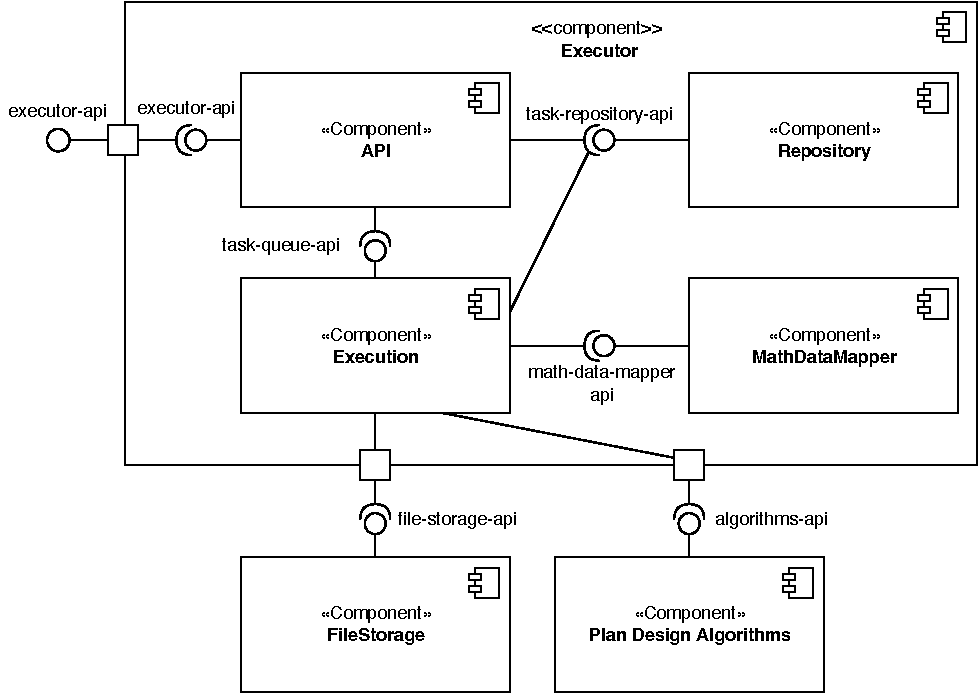
\includegraphics[scale=.6]{pictures/architecture/executor_component_common}
\end{figure}
\end{frame}

\begin{frame}
\frametitle{Компонент запуска математических методов}
\begin{figure}
    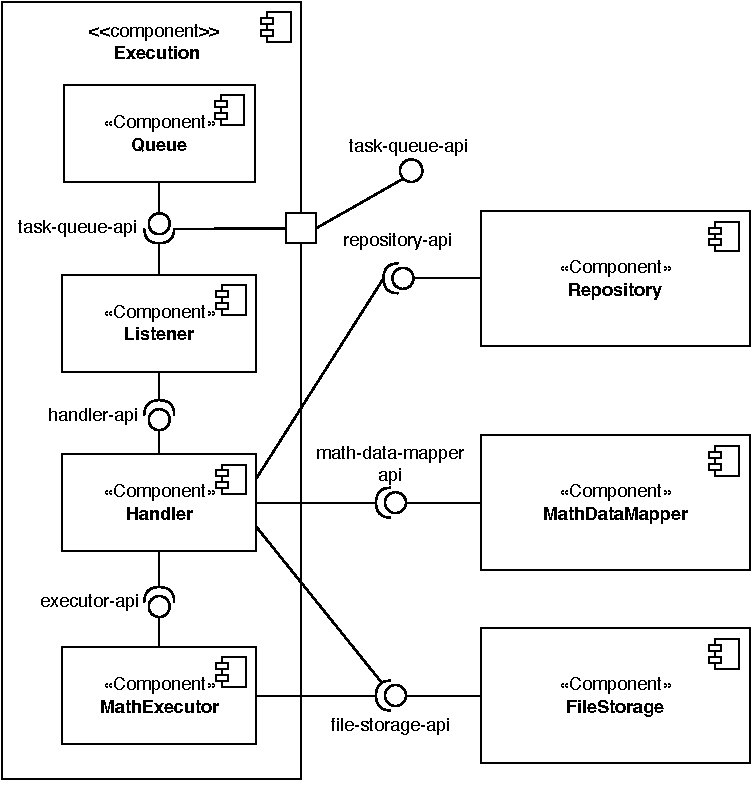
\includegraphics[scale=.5]{pictures/architecture/executor_component_detailed}
\end{figure}
\end{frame}

\begin{frame}
\frametitle{Хранилище расчётных данных}
\begin{figure}
    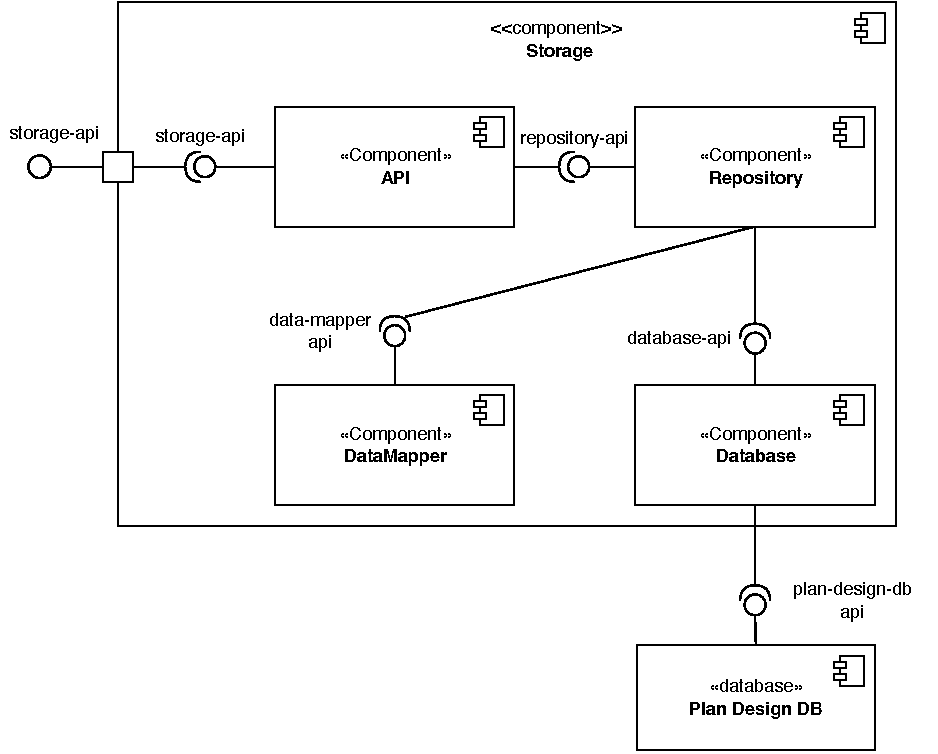
\includegraphics[scale=.55]{pictures/architecture/storage_component_common}
\end{figure}
\end{frame}
